\documentclass[12pt,a4paper]{article}
\usepackage[utf8]{inputenc}
\usepackage{amsmath}
\usepackage{amsfonts}
\usepackage{amssymb}
\usepackage[margin=2.5cm]{geometry}
\usepackage{graphicx}
\usepackage{caption}
\usepackage{subcaption}
\usepackage[nottoc,numbib]{tocbibind}
\title{Current-Voltage Characteristics of Weyl Semimetal Semiconducting Devices, Veselago Lenses and Hyperbolic Dirac Phase}
\author{R. D. Y. Hills, A. Kusmartseva and F. V. Kusmartsev}
\begin{document}
%%%%%
%%%%%
%%%%%
%%%%%
%%%%%
\maketitle
	\section{Supplementary Information}
	Here we present supplementary information for the paper titled "Current-Voltage Characteristics of Weyl Semimetal Transistors". The information here provides additional derivation for the calculations in the main text, which may be of interest to the reader.
%%%%%
%%%%%
%%%%%
%%%%%
%%%%%
		\subsection{Conservation of Probability Current}
		\label{Potential Step - Conservation of Probability Current}
			For the potential step the initial and final mediums are different. To allow for this the expression for transmission can be checked with the current continuity equation:
		\begin{equation}
			\frac{d}{dt}|\psi|^{2}+\nabla\cdot {\bf j}=0
		\end{equation}
		as the system here is time independent only the probability current;
		\begin{equation}
			{\bf j} =\psi^{*} {\bf \sigma} \psi
		\end{equation}
		needs to be considered. From the continuity equation; the probability current into the system must equal the probability current out of the system.
		\begin{align}
			j_{i}=j_{t}+j_{r}
			\hspace{1cm}
			1=\frac{j_{t}}{j_{i}}+\frac{j_{r}}{j_{i}}
		\end{align}
		By calculating the probability current both sides of the step the ratios of the transmitted and reflected current can be calculated. Using the eigenvectors derived previously the wave-functions on the left the step can be stated as:
		\begin{equation}
			\psi_{a}=
			\left[\begin{array}{ccc}
				\psi_{a1}\\
				\psi_{a2}
			\end{array}\right]
			=
			\left[\begin{array}{ccc}
				\left(e^{iq_{a}x}+re^{-iq_{a}x}\right)e^{ik_{y}y}e^{ik_{z}z}\\
				\left(\alpha_{a}e^{iq_{a}x+i\theta_{a}}-r\alpha_{a}e^{-iq_{a}x-i\theta_{a}}\right)e^{ik_{y}y}e^{ik_{z}z}
			\end{array}\right]
		\end{equation}
		where the incident and reflected components have been included. The subscript $a$ corresponds to region $a$ in Figure \ref{weyl-step}. The wave-functions on the right of the step (corresponding to region $b$ in Figure \ref{weyl-step}) only contain a transmitted component and is therefore given as:
		\begin{equation}
			\psi_{b}=
			\left[\begin{array}{ccc}
				\psi_{b1}\\
				\psi_{b2}
			\end{array}\right]
			=
			\left[\begin{array}{ccc}
				te^{iq_{b}x}e^{ik_{y}y}e^{ik_{z}z}\\
				t\alpha_{b}e^{iq_{b}x+i\theta_{b}}e^{ik_{y}y}e^{ik_{z}z}
			\end{array}\right]
		\end{equation}
		The groups of constants have been given the regional subscripts $a$ and $b$ to allow for different potentials in each region. For clarity these are defined as:
		\begin{align}
		q_{a}=\sqrt{\frac{\left(E-V_{a}\right)^{2}}{\hbar^{2}v_{f}^{2}}-k_{z}^{2}-k_{y}^{2}}\hspace{1cm}q_{b}=\sqrt{\frac{\left(E-V_{b}\right)^{2}}{\hbar^{2}v_{f}^{2}}-k_{z}^{2}-k_{y}^{2}}
		\end{align}
		\begin{align}
		\alpha_{a}=\frac{|E-V_{a}|sin\left(\phi_{a}\right)}{E-V_{a}+|E-V_{a}|cos\left(\phi_{a}\right)} \hspace{1cm} \alpha_{b}=\frac{|E-V_{b}|sin\left(\phi_{b}\right)}{E-V_{b}+|E-V_{b}|cos\left(\phi_{b}\right)}
		\end{align}
		\begin{align}
		\phi_{a}=arccos\left(\frac{\hbar v_{f} k_{z}}{|E-V_{a}|}\right)\hspace{1cm}\phi_{b}=arccos\left(\frac{\hbar v_{f} k_{z}}{|E-V_{b}|}\right)
		\end{align}
		\begin{align}
		\theta_{a}=arcsin\left(\frac{\hbar v_{f} k_{y}}{|E-V_{a}|sin\phi_{a}}\right)\hspace{1cm}\theta_{b}=arcsin\left(\frac{\hbar v_{f} k_{y}}{|E-V_{b}|sin\phi_{b}}\right)
		\end{align}
 		The probability current on the left of the step in the $x$-direction is then:
		\begin{align}
			\psi_{a}^{*} {\bf \sigma_{x}} \psi_{a}&=
			\left[\begin{array}{ccc}
				e^{-iq_{a}x}+r^{*}e^{iq_{a}x}&\alpha_{a}e^{-iq_{a}x-i\theta_{a}}-r^{*}\alpha_{a}e^{iq_{a}x+i\theta_{a}}
			\end{array}\right]
			\left[\begin{array}{ccc}
				0&1\\
				1&0
			\end{array}\right]
			\left[\begin{array}{ccc}
				e^{iq_{a}x}+re^{-iq_{a}x}\\
				\alpha_{a}e^{iq_{a}x+i\theta_{a}}-r\alpha_{a}e^{-iq_{a}x-i\theta_{a}}
			\end{array}\right]\\
			&=
			\left[\begin{array}{ccc}
				\alpha_{a}e^{-iq_{a}x-i\theta_{a}}-r^{*}\alpha_{a}e^{iq_{a}x+i\theta_{a}}&e^{-iq_{a}x}+r^{*}e^{iq_{a}x}
			\end{array}\right]
			\left[\begin{array}{ccc}
				e^{iq_{a}x}+re^{-iq_{a}x}\\
				\alpha_{a}e^{iq_{a}x+i\theta_{a}}-r\alpha_{a}e^{-iq_{a}x-i\theta_{a}}
			\end{array}\right]\\
			&=
			2\alpha_{a}cos\left(\theta_{a}\right)-2|r|^{2}\alpha_{a}cos\left(\theta_{a}\right)
			\label{left}
		\end{align}
		and on the right side:
		\begin{align}
			\psi_{b}^{*} {\bf \sigma_{x}} \psi_{b}&=
			\left[\begin{array}{ccc}
				t^{*}e^{-iq_{b}x}&t^{*}\alpha_{b}e^{-iq_{b}x-i\theta_{b}}
			\end{array}\right]
			\left[\begin{array}{ccc}
				0&1\\
				1&0
			\end{array}\right]
			\left[\begin{array}{ccc}
				te^{iq_{b}x}\\
				t\alpha_{b}e^{iq_{b}x+i\theta_{b}}
			\end{array}\right]\\
			&=
			2|t|^{2}\alpha_{b}cos\left(\theta_{b}\right)
			\label{right}
		\end{align}
		Current on the left side of the step must then equal current on the right of the step. Equating Equation (\ref{left}) and Equation (\ref{right}) produces:
		\begin{equation}
			1=|t|^{2}\frac{\alpha_{b}cos\left(\theta_{b}\right)}{\alpha_{a}cos\left(\theta_{a}\right)}+|r|^{2}
		\end{equation}
		Showing that the normal method of using $|t|^{2}$ as the transmission probability does not hold for asymmetrical systems. With this modification the transmission can now be found by:
		\begin{equation}
			T=1-R
			\hspace{1cm}
			T=|t|^{2}\frac{\alpha_{b}cos\left(\theta_{b}\right)}{\alpha_{a}cos\left(\theta_{a}\right)}
			\label{newT}
		\end{equation}
		However if $\alpha_{a}$ and $\theta_{a}$ are equal to $\alpha_{b}$ and $\theta_{b}$, as with the symmetrical barrier case, the current conservation produces $1=|t|^{2}+|r|^{2}$ and transmission can be calculated normally.
%%%%%
%%%%%
%%%%%
%%%%%
%%%%%
		\subsection{The Potential Step}
		\begin{figure}
			\centerline{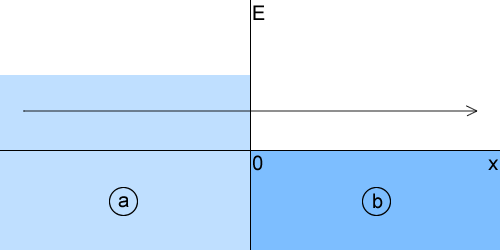
\includegraphics[scale=0.6]{images/weyl-step}}
			\caption{The potential step centered at $x=0$ with $V_{a}\neq 0$ and $V_{b}=0$.}
			\label{weyl-step}
		\end{figure}
		The system in Figure \ref{weyl-step} can be described with the previously derived wave-functions as a set of simultaneous equations. Continuity at the barrier interface causes the wave-functions on the left and right of the step to be equal:
		\begin{align}
			e^{ik_{z}z}e^{ik_{y}y}\left(e^{iq_{a}x}+re^{-iq_{a}x}\right)&=te^{iq_{b}x}e^{ik_{y}y}e^{ik_{z}z}\\
			e^{ik_{z}z}e^{ik_{y}y}\left(\alpha_{a}e^{iq_{a}x+i\theta_{a}}-r\alpha_{a}e^{-iq_{a}x-i\theta_{a}}\right)&=t\alpha_{b}e^{iq_{b}x+i\theta_{b}}e^{ik_{y}y}e^{ik_{z}z}
		\end{align}
		The subscripts $a$ and $b$ represent constants for the corresponding region in Figure \ref{weyl-step}. By setting the boundary between the two regions as $x=0$:
		\begin{align}
			1+r&=t\\
			\alpha_{a}e^{i\theta_{a}}-r\alpha_{a}e^{-i\theta_{a}}&=t\alpha_{b}e^{i\theta_{b}}
		\end{align}
		and solving for $t$:
		\begin{equation}
			t=\frac{2\alpha_{a}cos\left(\theta_{a}\right)}{\alpha_{a}e^{-i\theta_{a}}+\alpha_{b}e^{i\theta_{b}}}
		\end{equation}
		an expression for $|t|^{2}$ is then:
		\begin{equation}
			|t|^{2}=\frac{4\alpha_{a}^{2}cos^{2}\left(\theta_{a}\right)}{\alpha_{a}^{2}+\alpha_{b}^{2}+2\alpha_{a}\alpha_{b}cos\left(\theta_{a}+\theta_{b}\right)}
		\end{equation}
		However, from Section \ref{Potential Step - Conservation of Probability Current}, it is known that the transmission through the step is not simply $|t|^{2}$. With Equation (\ref{newT}); the expression for transmission from the conservation of current calculation the transmission through the step becomes:
		\begin{equation}
			T=\frac{4\alpha_{a}\alpha_{b}cos\left(\theta_{a}\right)cos\left(\theta_{b}\right)}{\alpha_{a}^{2}+\alpha_{b}^{2}+2\alpha_{a}\alpha_{b}cos\left(\theta_{a}+\theta_{b}\right)}
		\end{equation}
%%%%%
%%%%%
%%%%%
%%%%%
%%%%%
		\subsection{The Potential Barrier}
		\label{weyl - Scattering Properties}
		\begin{figure}[h]
			\centerline{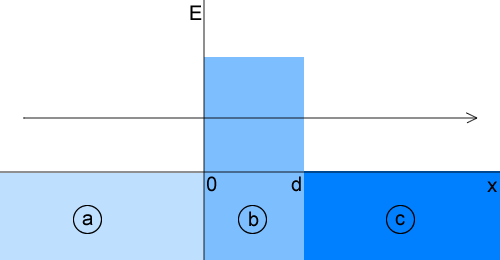
\includegraphics[scale=0.7]{images/weyl-symmetrical-flat}}
			\caption{The potential barrier problem. A potential barrier is placed in the $x$-direction with a height $V_{b}$ and a width $d$. The shaded region shows where hole transport is present. The three independent regions have been labled as $a,b$ and $c$.}
			\label{weyl-symmetrical-flat}
		\end{figure}
		The wave-functions previously derived can then be used in the scattering problem described in Figure \ref{weyl-symmetrical-flat}. Here regional subscripts will be added to groups of constants. For the transfer matrix method \cite{b18} left and right travelling waves are considered in all regions so that the wave-functions in each region can be defined as:
		\begin{align}
			\psi_{a}&=
			\left[\begin{array}{ccc}
				\psi_{a1}\\
				\psi_{a2}
			\end{array}\right]
			=
			\left[\begin{array}{ccc}
				\left(a_{1}e^{iq_{a}x}+a_{2}e^{-iq_{a}x}\right)e^{ik_{y}y}e^{ik_{z}z}\\
				\left(a_{1}\alpha_{a}e^{iq_{a}x+i\theta_{a}}-a_{2}\alpha_{a}e^{-iq_{a}x-i\theta_{a}}\right)e^{ik_{y}y}e^{ik_{z}z}
			\end{array}\right]
			\\
			\psi_{b}&=
			\left[\begin{array}{ccc}
				\psi_{b1}\\
				\psi_{b2}
			\end{array}\right]
			=
			\left[\begin{array}{ccc}
				\left(a_{3}e^{iq_{b}x}+a_{4}e^{-iq_{b}x}\right)e^{ik_{y}y}e^{ik_{z}z}\\
				\left(a_{3}\alpha_{b}e^{iq_{b}x+i\theta_{b}}-a_{4}\alpha_{b}e^{-iq_{b}x-i\theta_{b}}\right)e^{ik_{y}y}e^{ik_{z}z}
			\end{array}\right]
			\\
			\psi_{c}&=
			\left[\begin{array}{ccc}
				\psi_{c1}\\
				\psi_{c2}
			\end{array}\right]
			=
			\left[\begin{array}{ccc}
				\left(a_{5}e^{iq_{a}x}+a_{6}e^{-iq_{a}x}\right)e^{ik_{y}y}e^{ik_{z}z}\\
				\left(a_{5}\alpha_{a}e^{iq_{a}x+i\theta_{a}}-a_{6}\alpha_{a}e^{-iq_{a}x-i\theta_{a}}\right)e^{ik_{y}y}e^{ik_{z}z}
			\end{array}\right]
		\end{align}
Continuity of the wave-functions requires that at the first barrier interface $\psi_{a}=\psi_{b}$. As the barrier interface is located at $x=0$ the wave-functions reduce to:
		\begin{align}
			\left[\begin{array}{ccc}
				1&1\\
				\alpha_{a}e^{i\theta_{a}}&-\alpha_{a}e^{-i\theta_{a}}
			\end{array}\right]
			\left[\begin{array}{ccc}
				a_{1}\\
				a_{2}
			\end{array}\right]
			&=
			\left[\begin{array}{ccc}
				1&1\\
				\alpha_{b}e^{i\theta_{b}}&-\alpha_{b}e^{-i\theta_{b}}
			\end{array}\right]
			\left[\begin{array}{ccc}
				a_{3}\\
				a_{4}
			\end{array}\right]\\
			m_{1}\left[\begin{array}{ccc}
				a_{1}\\
				a_{2}
			\end{array}\right]
			&=
			m_{2}\left[\begin{array}{ccc}
				a_{3}\\
				a_{4}
			\end{array}\right]
		\end{align}
		For convenience the matrices $m_{1}, m_{2}, m_{3}, m_{4}$ have been introduced as the corresponding wave-function in matrix form. At the second boundary $x=d$ the continuity requires that $\psi_{b}=\psi_{c}$ resulting in:
		\begin{align}
			\left[\begin{array}{ccc}
				e^{iq_{b}d}&e^{-iq_{b}d}\\
				\alpha_{b}e^{iq_{b}d+i\theta_{b}}&-\alpha_{b}e^{-iq_{b}d-i\theta_{b}}
			\end{array}\right]
			\left[\begin{array}{ccc}
				a_{3}\\
				a_{4}
			\end{array}\right]
			&=
			\left[\begin{array}{ccc}
				e^{iq_{a}d}&e^{-iq_{a}d}\\
				\alpha_{a}e^{iq_{a}d+i\theta_{a}}&-\alpha_{a}e^{-iq_{c}d-i\theta_{a}}
			\end{array}\right]
			\left[\begin{array}{ccc}
				a_{5}\\
				a_{6}
			\end{array}\right]\\
			m_{3}\left[\begin{array}{ccc}
				a_{3}\\
				a_{4}
			\end{array}\right]
			&=
			m_{4}\left[\begin{array}{ccc}
				a_{5}\\
				a_{6}
			\end{array}\right]
		\end{align}
		The transfer matrix $M$ can then be obtained by eliminating constants $a_{3}$ and $a_{4}$ so that:
		\begin{align}
			\left[\begin{array}{ccc}
				a_{5}\\
				a_{6}
			\end{array}\right]=M
			\left[\begin{array}{ccc}
				a_{1}\\
				a_{2}
			\end{array}\right]\hspace{1cm}
			M=m_{4}^{-1}m_{3}m_{2}^{-1}m_{1}
		\end{align}
		Evaluating the transfer matrix allows the transmission coefficient and the total transmission to be obtained. From transfer matrix theory $t=1/M_{2,2}$ and $T=|t|^{2}$ resulting in:
		\begin{equation}
			t=\frac{2\alpha_{a}\alpha_{b}e^{-idq_{a}}cos\left(\theta_{a}\right)cos\left(\theta_{b}\right)}{2\alpha_{a}\alpha_{b}\left(cos\left(dq_{b}\right)cos\left(\theta_{a}\right)cos\left(\theta_{b}\right)+isin\left(dq_{b}\right)sin\left(\theta_{a}\right)sin\left(\theta_{b}\right)\right)-isin\left(dq_{b}\right)\left(\alpha_{a}^{2}+\alpha_{b}^{2}\right)}
		\end{equation}
		\begin{equation}
			T=\frac{4\alpha_{a}^{2}\alpha_{b}^{2}cos^{2}\left(\theta_{a}\right)cos^{2}\left(\theta_{b}\right)}{4\alpha_{a}^{2}\alpha_{b}^{2}cos^{2}\left(dq_{b}\right)cos^{2}\left(\theta_{a}\right)cos^{2}\left(\theta_{b}\right)+sin^{2}\left(dq_{b}\right)\left(2\alpha_{a}\alpha_{b}sin\left(\theta_{a}\right)sin\left(\theta_{b}\right)-\alpha_{a}^{2}-\alpha_{b}^{2}\right)^{2}}
		\label{weyl-combo-t}
		\end{equation}
		This equation can then be reduced to produce the transmission results for two-dimensional systems. To remove $k_{z}$ the angles $\phi_{a,b}$ can be set to $\pi /2$ resulting in:
		\begin{equation}
			T=\frac{4s_{a}^{2}s_{b}^{2}cos^{2}\left(\theta_{a}\right)cos^{2}\left(\theta_{b}\right)}{4s_{a}^{2}s_{b}^{2}cos^{2}\left(dq_{b}\right)cos^{2}\left(\theta_{a}\right)cos^{2}\left(\theta_{b}\right)+sin^{2}\left(dq_{b}\right)\left(2s_{a}s_{b}sin\left(\theta_{a}\right)sin\left(\theta_{b}\right)-s_{a}^{2}-s_{b}^{2}\right)^{2}}
		\end{equation}
		where $s_{a,b}=sgn\left(E-V_{a,b}\right)$. Similarly the $k_{y}$ dependence can be removed from Equation  (\ref{weyl-combo-t}) by setting the angles $\theta_{a,b}=0$. Therefore the result for a two-dimensional material in the $x-z$ plane takes the form:
		\begin{equation}
			T=\frac{4\alpha_{a}^{2}\alpha_{b}^{2}}{4\alpha_{a}^{2}\alpha_{b}^{2}cos^{2}\left(dq_{b}\right)+sin^{2}\left(dq_{b}\right)\left(\alpha_{a}^{2}+\alpha_{b}^{2}\right)^{2}}
		\label{weyl-combo-t}
		\end{equation}

%%%%%
%%%%%
%%%%%
%%%%%
%%%%%

	\subsection{Transfer Matrix in Optics}
	\label{optics}
		In optics an electromagnetic wave can be expressed as:
		\begin{equation}
			\psi=c_{1}e^{ikx}+c_{2}e^{-ikx}
		\end{equation}
		where $k$ is the wave number equivalent to $2\pi/\lambda$. When incident on a boundary the wave and the spacial derivitive must be continuous.
		\begin{equation}
			\frac{d}{dx}\psi=c_{1}ike^{ikx}-c_{2}ike^{-ikx}
		\end{equation}
		When the boundary separates mediums; the wave must change within the medium so that:
		\begin{equation}
			\psi=c_{3}e^{iqx}+c_{4}e^{-iqx}
		\end{equation}
		where $q=nk$ and $n$ is the refractive index of the new medium. 
		\begin{figure}[h]
			\centerline{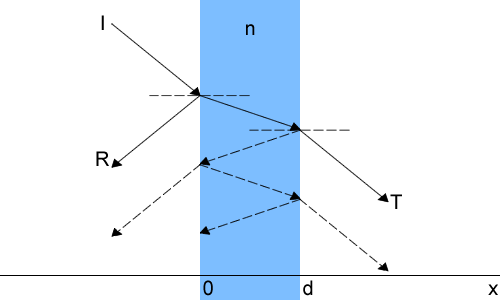
\includegraphics[scale=0.5]{images/optics-barrier-flat}}
			\caption{Diagram of an electromagnetic wave entering a region with refractive index $n$. The incident (I), reflected (R) and transmitted (T) probabilties are shown for a region of width $d$.}
			\label{optics-barrier-flat}
		\end{figure}
		The transfer matrix for the wave passing through some medium can now be constructed. The waves in matrix form for each region are defined as:
		\begin{align}
			\psi_{a}&=
			\left[\begin{array}{ccc}
				e^{ikx}&e^{-ikx}\\
				ike^{ikx}&-ike^{-ikx}
			\end{array}\right]
			\left[\begin{array}{ccc}
				c_{1}\\
				c_{2}
			\end{array}\right]
			\\
			\psi_{b}&=
			\left[\begin{array}{ccc}
				e^{iqx}&e^{-iqx}\\
				iqe^{iqx}&-iqe^{-iqx}
			\end{array}\right]
			\left[\begin{array}{ccc}
				c_{3}\\
				c_{4}
			\end{array}\right]
			\\
			\psi_{c}&=
			\left[\begin{array}{ccc}
				e^{ikx}&e^{-ikx}\\
				ike^{ikx}&-ike^{-ikx}
			\end{array}\right]
			\left[\begin{array}{ccc}
				c_{5}\\
				c_{6}
			\end{array}\right]
		\end{align}
		At the first boundary at $x=0$ the waves $\psi_{a}$ and $\psi_{b}$ must be continuous and therefore $\psi_{a}=\psi_{b}$, which may be written as:
		\begin{align}
			\left[\begin{array}{ccc}
				c_{3}\\
				c_{4}
			\end{array}\right]
			&=
			\left[\begin{array}{ccc}
				1&1\\
				iq&-iq
			\end{array}\right]^{-1}
			\left[\begin{array}{ccc}
				1&1\\
				ik&-ik
			\end{array}\right]
			\left[\begin{array}{ccc}
				c_{1}\\
				c_{2}
			\end{array}\right]
			\\&=
			\frac{1}{2q}\left[\begin{array}{ccc}
				q+k&q-k\\
				q-k&q+k
			\end{array}\right]
			\left[\begin{array}{ccc}
				c_{1}\\
				c_{2}
			\end{array}\right]
			\\&=
			m_{1}\left[\begin{array}{ccc}
				c_{1}\\
				c_{2}
			\end{array}\right]
		\end{align}
		At the second boundary at $x=d$ the wave $\psi_{b}$ must be continuous with $\psi_{c}$ and therefore $\psi_{b}=\psi_{c}$. This will be expressed as:
		\begin{align}
			\left[\begin{array}{ccc}
				c_{5}\\
				c_{6}
			\end{array}\right]
			&=
			\left[\begin{array}{ccc}
				e^{ikd}&e^{-ikd}\\
				ike^{ikd}&-ike^{-ikd}
			\end{array}\right]^{-1}
			\left[\begin{array}{ccc}
				e^{iqd}&e^{-iqd}\\
				iqe^{iqd}&-iqe^{-iqd}
			\end{array}\right]
			\left[\begin{array}{ccc}
				c_{3}\\
				c_{4}
			\end{array}\right]
			\\&=
			\frac{1}{2k}\left[\begin{array}{ccc}
				\left(k+q\right)e^{-ikd+iqd}&\left(k-q\right)e^{-ikd-iqd}\\
				\left(k-q\right)e^{ikd+iqd}&\left(k+q\right)e^{ikd-iqd}
			\end{array}\right]
			\left[\begin{array}{ccc}
				c_{3}\\
				c_{4}
			\end{array}\right]
			\\&=
			m_{2}\left[\begin{array}{ccc}
				c_{3}\\
				c_{4}
			\end{array}\right]
		\end{align}
		The transfer matrix relating the final wave amplitudes to the incident wave amplitudes can finally be expressed as:
		\begin{align}
			\left[\begin{array}{ccc}
				c_{3}\\
				c_{4}
			\end{array}\right]
			=m_{2}m_{1}
			\left[\begin{array}{ccc}
				c_{1}\\
				c_{2}
			\end{array}\right]
		\end{align}
		Here the transfer matrix $M$ is defined as:
		\begin{align}
			M&=m_{2}m_{1}
			\\&=\frac{1}{4kq}
			\left[\begin{array}{ccc}
				\left(k+q\right)e^{-ikd+iqd}&\left(k-q\right)e^{-ikd-iqd}\\
				\left(k-q\right)e^{ikd+iqd}&\left(k+q\right)e^{ikd-iqd}
			\end{array}\right]
			\left[\begin{array}{ccc}
				q+k&q-k\\
				q-k&q+k
			\end{array}\right]
			\\&=\frac{1}{2kq}
			\left[\begin{array}{ccc}
				\left(2kqcos\left(qd\right)+i\left(k^{2}+q^{2}\right)sin\left(qd\right)\right)e^{-ikd}&\left(i\left(q^{2}-k^{2}\right)sin\left(qd\right)\right)e^{-ikd}\\
				\left(i\left(k^{2}-q^{2}\right)sin\left(qd\right)\right)e^{ikd}&\left(2kqcos\left(qd\right)-i\left(k^{2}+q^{2}\right)sin\left(qd\right)\right)e^{ikd}
			\end{array}\right]
		\end{align}
		The transmission probability though the intermediate medium is then taken as:
		\begin{equation}
			T=\frac{1}{|M_{22}|^{2}}
			=\frac{4k^{2}q^{2}}{4k^{2}q^{2}cos^{2}\left(qd\right)+\left(k^{2}+q^{2}\right)^{2}sin^{2}\left(qd\right)}
		\end{equation}
		With the resonance condition of $T=1$ occuring when:
		\begin{equation}
			dq=n\pi
		\end{equation}
		With the equations for electromagnetic waves:
		\begin{equation}
			k=\frac{2\pi}{\lambda}
			\hspace{1cm}
			c=f\lambda
			\hspace{1cm}
			E=hf
		\end{equation}
		where $c$ is the speed of light in a vacuum, $h$ is the plank constant, $f$ is the frequency of the wave and $\lambda$ is the wavelength. With these definitions the wave number can be expressed in terms of the energy $E$:
		\begin{equation}
			k=\frac{E}{\hbar c}
		\end{equation}
		The transmission probability can also be expressed in terms of energy:
		\begin{equation}
			T=\frac{4n^{2}}{4n^{2}cos^{2}\left(\frac{dnE}{\hbar c}\right)+\left(1+n^{2}\right)^{2}sin^{2}\left(\frac{dnE}{\hbar c}\right)}
		\end{equation}
		with the resonance condition:
		\begin{equation}
			\frac{dnE}{\hbar c}=n_{r}\pi
		\end{equation}

%%%%%
%%%%%%%%%%
%%%%%
		\section{Landauer Formalism in Weyl Semimetals}
			In this section the Landauer formalism is derived for a Weyl semimetal scattering device. For a single channel system at non-zero temperatures the current through the system shown in Figure \ref{introduction-current} can be found [].
			\begin{figure}[h]
				\centerline{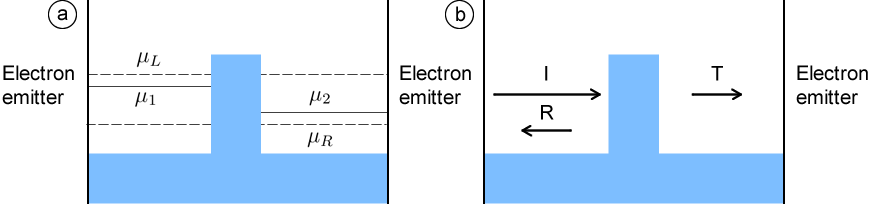
\includegraphics[scale=0.5]{current}}
				\caption{(Colour Online) (a) Diagram showing quasi-Fermi-energies and chemical potentials of the perfectly conducting wires. Here the left emitter injects electrons up to the quasi-Fermi-energy $\mu_{L}$ and the right emitter injects electrons up the the quasi-Fermi-energy $\mu_{R}$. $\mu_{1}$ and $\mu_{2}$ are the chemical potentials of the perfectly conducting wires to the left and right of the scattering device. (b) A scattering device between two electron emitters. Charge carriers from the left emitter are scattered with a probability $R$ of being reflected and probability $T$ or transmitting through the scattering device.}
				\label{introduction-current}
			\end{figure}
			 The system in Figure \ref{introduction-current} consists of 2 incoherent electron reservoirs, which emit charge carriers up to the quasi-Fermi-energy $\mu_{L,R}$, where the subscript $L$ and $R$ represent the reservoir at left or right side of the system respectivly. These reservoirs are then connected to a scattering device via perfect and identical one dimensional conductors. These conductors have chemical potentials $\mu_{1}$ and $\mu_{2}$. The current leaving the left reservoir is then:
			\begin{equation}
				I=ev_{f}\frac{dn}{dE}\left(\mu_{L}-\mu_{R}\right)
				\label{current-dos}
			\end{equation}
			where $e$ is the electron charge, $v_{f}$ is the Fermi velocity and $dn/dE$ is the density of states. The current that is transmitted through the sample is then:
			\begin{equation}
				I=ev_{f}\frac{dn}{dE}T\left(\mu_{R}-\mu_{R}\right)
				\label{current-transmit}
			\end{equation}
			where $T$ is the transmission probability through the scattering device. The density of states for Weyl semimetals at a Dirac point is given by:
			\begin{equation}
				\rho\left(E\right)=\frac{L_{x}L_{y}L_{z}}{\pi\hbar^{3}v_{f}^{3}}E^{2}
				\label{weyl-dos}
			\end{equation}
			Where  $L_{x}, L_{y}$ is the size of the sample in the respective dimension. As only the $x$-direction current will be considered here, the current in the $x$-direction will be the same in each cell, therefore only size of the system in the $y$-direction will affect the $x$-directional current. This way the quantity $L_{x}$ can be set to one and removed from the calculation. The current through the sample from equation (\ref{current-transmit}) in the $x$-direction becomes:
			\begin{equation}
				I_{x}=e\frac{L_{y}L_{z}}{\pi\hbar^{3}v_{f}^{2}}T\left(E,\theta, \phi\right)\left(\mu_{L}-\mu_{R}\right)E^{2}cos\left(\theta\right)sin\left(\psi\right)
			\end{equation}
			The energy and angular dependence for $T$ has been included here to allow for the Weyl semimetal transmission probability. At non-zero temperatures the states are instead filled according to the corresponding Fermi-Dirac distribution.
			\begin{equation}
				f_{L,R}=f\left(E-\mu_{L,R}\right)=\frac{1}{e^{\frac{E-\mu_{L,R}}{k_{b}t}}+1}
			\end{equation}
			The current must then be integrated over all energies and incident angles to account for all states in the Fermi-Dirac distributions.
			\begin{equation}
				I_{x}=I_{0}\int^{\infty}_{-\infty}\int^{\pi/2}_{-\pi/2}\int^{\pi}_{0}T\left(E,\theta, \phi\right)\left[f_{L}-f_{R}\right]E^{2}cos\left(\theta\right)sin\left(\phi\right)dEd\theta d\phi
			\end{equation}
			with the constant $I_{0}=e\frac{2L_{y}L_{z}}{\pi\hbar^{3}v_{f}^{2}}$. 
%%%%%
%%%%%
%%%%%
%%%%%
%%%%%

\begin{thebibliography}{10}

\bibitem{b18}
Wave Propagation: From Electrons to Photonic Crystals and Left-Handed Materials,
P. Markos and C. M. Soukoulis,
\newblock Princeton University Press, 1 Apr 2008

\end{thebibliography}

\end{document}